% Please use the skeleton file you have received in the
% invitation-to-submit email, where your data are already
% filled in. Otherwise please make sure you insert your
% data according to the instructions in PoSauthmanual.pdf
\documentclass[a4paper]{jpconf}
\usepackage{graphicx}

\begin{document}

\title{Liquid Argon optical properties to be used in Geant4 and Opticks Simulations}

\author{ Hans~Wenzel$^1$}

\address{ $^1$~Fermilab PO Box 500, Batavia, IL 60510,
USA}

\ead{wenzel@fnal.gov}

\begin{abstract}
  In Geant4 and Opticks optical properties like e.g. the materials refractive
  index are inputs that have to be provided. In this paper we collect the
  optical properties relevant for liquid Argon TPC's.  
\end{abstract}

\section{Introduction}
optical properties given as
\begin{verbatim}
Light yield ~ few 10,000’s of photons per MeV (depends on E field, particle type and purity)
(SCINTILLATIONYIELD: 50000/MeV when no electric field present)
Wavelength of emission is 128nm (FWHM= 10nm)

Light with two characteristic time constants:
- fast component  (SCINTILLATIONTIMECONSTANT1): 6 ns  
  	     	              (SCINTILLATIONYIELD1): 0.75

- slow component (SCINTILLATIONTIMECONSTANT2): 1500 ns
				 (SCINTILLATIONYIELD2): 0.25
(RESOLUTIONSCALE): 1

Refraction Index: n = 1.358 ± 0.003 at 128 nm (M. Babicz et al 2020 JINST 15 P09009)
                            ( compared to n= 1.45 ± 0.07 (ArXiv:1502.04213))
Group velocity: 1/ vg = 7.46 ± 0.08 ns/m at 128 nm

Argon is highly transparent to its own scintillation light. (ABSLENGTH)
  >1.1 m (ArXiv:1511.07725) 
Rayleigh scattering length (RAYLEIGH): 90 cm (M. Babicz et al 2020 JINST 15 P09009)
                                                                55+/- 5 cm (ArXiv:1502.04213)

\end{verbatim}



\section{Requirements}

\begin{figure}[ht]
\begin{center}
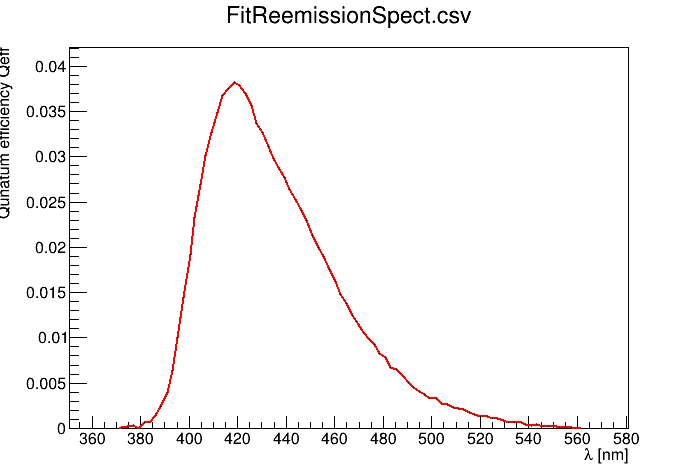
\includegraphics[width=35.5pc]{wls.epsf}
\end{center}
\caption{\label{fig1}wave length spectrum.}
\end{figure}



\section{Conclusions and Outlook}
DoSSiER provides a repository to collect and organize validation and regression test results and
the experimental data used for physics validation tests. The  web application component of DoSSiER allows easy access 
to the information for members of simulation collaborations and the general user community. 
The  web service component allows for programmatic access to the data
stored in DoSSiER.\@ 
We are in the process of adding new tests and experimental data to the repository. 
Originally we concentrated on Geant4 tests of hadronic and electromagnetic physics that are of interest for high energy physics 
experiments, but in the future we plan to include tests that are of interest in other areas such as medical and space science. Also
we are in the process of adding GEANIE and GeantV data in cooperation with the respective collaborations.
The website front-page (currently reachable at
\verb"http://g4devel.fnal.gov:8080/DoSSiER/") is already available to
the general public interested in providing feedback. 
Additional data-sets and simulation results are
expected in the near future and we plan to improve the website
based on the comments of the first users in the next few years, the
current priority being the extension of included simulations and data.
With the
addition of more data we expect that this tool will become the
main entry point to serve as result repository for both higher level
(e.g.\@ shower shapes in calorimeters) and microscopic (e.g.\@
cross-sections, final state multiplicities) validations. To achieve this
goal we are working in close collaboration with simulation experts. 
 \section*{References}

\begin{thebibliography}{99}
\bibitem{ref:Geant4-4}
 Allison J et al. 2016 {\it Nuclear Instruments and Methods in Physics
                Research A} {\bf 835} (186--225).
\bibitem{ref:GeantV}
 \verb|http://geant.cern.ch/|.
\bibitem{inspire} High-Energy Physics Literature Database,
  \verb"http://inspirehep.net"/.
\bibitem{scripts}  
  \verb''https://github.com/hanswenzel/CaTS/tree/master/scripts/LAr.C''/.
  \verb''https://github.com/hanswenzel/CaTS/tree/master/scripts/wls.C''/.

\bibitem{wls} Christopher Benson, Gabriel D. Orebi Gann, Victor Gehman
  {\it Measurements of the intrinsic quantum efficiency and absorption
      length of tetraphenyl butadiene thin films in the vacuum
      ultraviolet regime}
Eur. Phys. J. C (2018) 78:329
\bibitem{grace}Emily Grace, Alistair Butcher, Jocelyn Monroe, James A. Nikkel
  \it{Index of refraction, Rayleigh scattering length, and Sellmeier coefficients in solid and liquid argon and xenon}
  \verb'' ArXiv:1502.04213''/
\bibitem{gv} 
  \it{A measurement of the group velocity of scintillation light in liquid argon}
  M. Babicz et al 2020 JINST 15 P09009
\bibitem{ben}
  Ben Jones, \it{Introduction to Scintillation Light in Liquid Argon}
  \verb''http://microboone-exp.fnal.gov''/
  \bibitem{morikawa}E. Morikawa, R. Reininger, P. Gürtler, V. Saile, and P. Laporte
\it{Argon, krypton, and xenon excimer luminescence: From the dilute gas to the
condensed phase}
J. Chem. Phys. 91, 1469 (1989);
  \verb''https://doi.org/10.1063/1.457108''/


  
\end{thebibliography}

\end{document}
